\documentclass{standalone}
\usepackage{tikz}
\usetikzlibrary{patterns, positioning}

\begin{document}
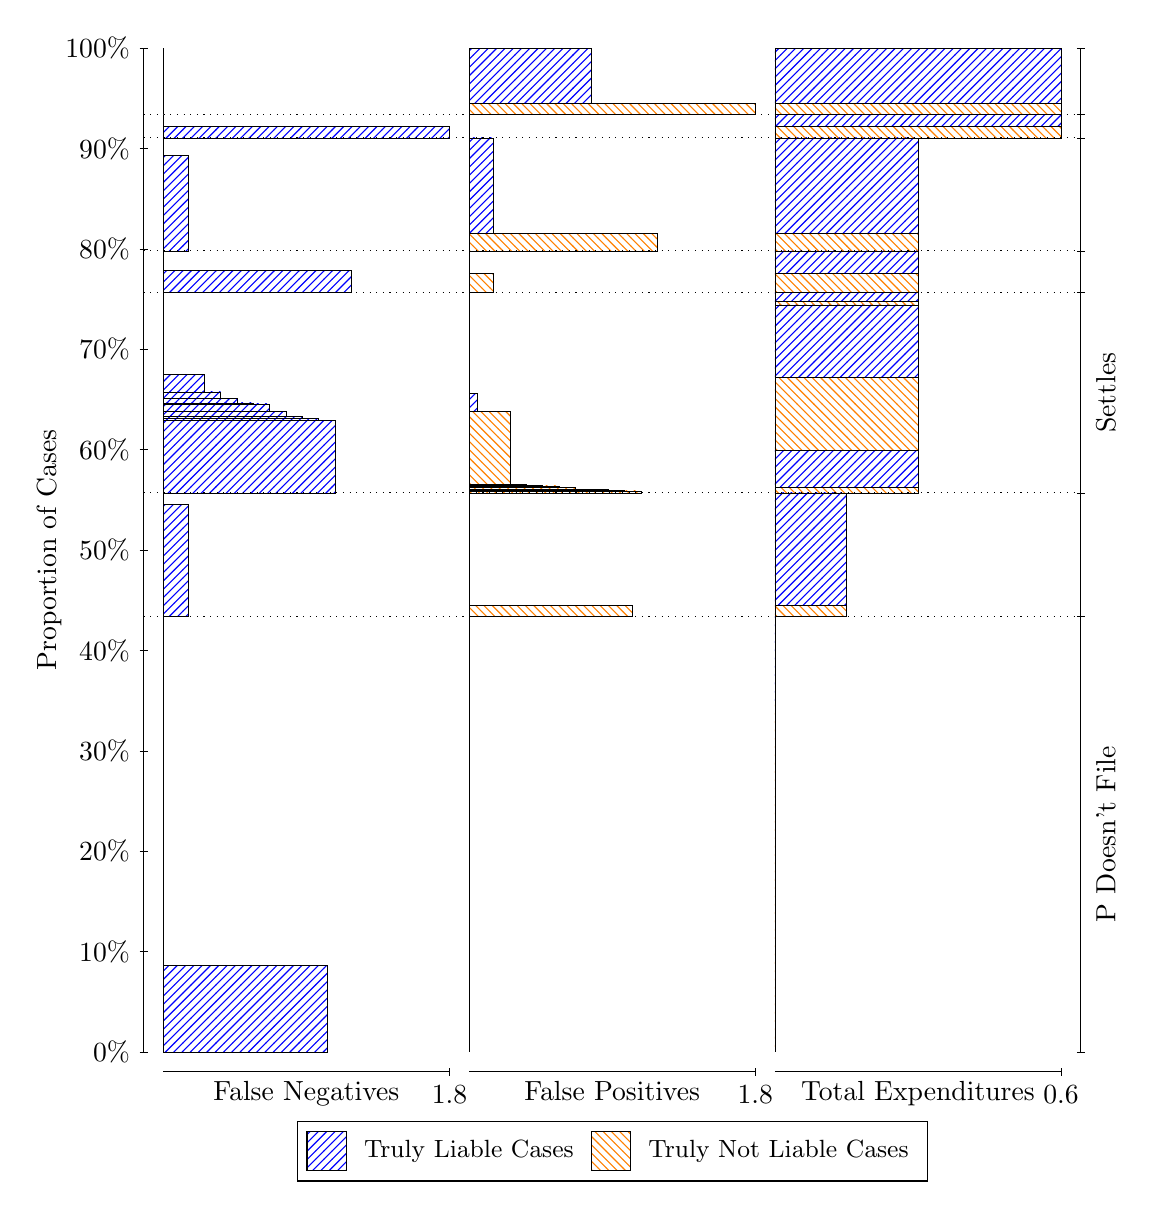
\begin{tikzpicture}
\draw[black, very thin] (1.5,1.75) -- (1.5,14.5);
\node[rotate=90, anchor=center] at (0.3, 8.125) {Proportion of Cases};
\draw[black, very thin] (1.45,1.75) -- (1.55,1.75);
\node[anchor=east] at (1.45, 1.75) {0\%};
\draw[black, very thin] (1.45,3.025) -- (1.55,3.025);
\node[anchor=east] at (1.45, 3.025) {10\%};
\draw[black, very thin] (1.45,4.3) -- (1.55,4.3);
\node[anchor=east] at (1.45, 4.3) {20\%};
\draw[black, very thin] (1.45,5.575) -- (1.55,5.575);
\node[anchor=east] at (1.45, 5.575) {30\%};
\draw[black, very thin] (1.45,6.85) -- (1.55,6.85);
\node[anchor=east] at (1.45, 6.85) {40\%};
\draw[black, very thin] (1.45,8.125) -- (1.55,8.125);
\node[anchor=east] at (1.45, 8.125) {50\%};
\draw[black, very thin] (1.45,9.4) -- (1.55,9.4);
\node[anchor=east] at (1.45, 9.4) {60\%};
\draw[black, very thin] (1.45,10.675) -- (1.55,10.675);
\node[anchor=east] at (1.45, 10.675) {70\%};
\draw[black, very thin] (1.45,11.95) -- (1.55,11.95);
\node[anchor=east] at (1.45, 11.95) {80\%};
\draw[black, very thin] (1.45,13.225) -- (1.55,13.225);
\node[anchor=east] at (1.45, 13.225) {90\%};
\draw[black, very thin] (1.45,14.5) -- (1.55,14.5);
\node[anchor=east] at (1.45, 14.5) {100\%};

\draw[black, very thin] (13.4,1.75) -- (13.4,14.5);
\draw[black, very thin] (13.35,1.75) -- (13.45,1.75);
\node[anchor=west] at (13.35, 1.75) {};
\draw[black, very thin] (13.35,7.2812) -- (13.45,7.2812);
\node[anchor=west] at (13.35, 7.2812) {};
\draw[black, very thin] (13.35,8.8513) -- (13.45,8.8513);
\node[anchor=west] at (13.35, 8.8513) {};
\draw[black, very thin] (13.35,11.395) -- (13.45,11.395);
\node[anchor=west] at (13.35, 11.395) {};
\draw[black, very thin] (13.35,11.923) -- (13.45,11.923);
\node[anchor=west] at (13.35, 11.923) {};
\draw[black, very thin] (13.35,13.359) -- (13.45,13.359);
\node[anchor=west] at (13.35, 13.359) {};
\draw[black, very thin] (13.35,13.653) -- (13.45,13.653);
\node[anchor=west] at (13.35, 13.653) {};
\draw[black, very thin] (13.35,14.5) -- (13.45,14.5);
\node[anchor=west] at (13.35, 14.5) {};

\draw[black, very thin, pattern color=blue, pattern=north east lines] (1.75,1.75) rectangle (3.8262,2.8499);
\draw[black, very thin, pattern color=orange, pattern=north west lines] (1.75,2.8499) rectangle (1.75,7.2812);
\draw[black, very thin, pattern color=blue, pattern=north east lines] (1.75,7.2812) rectangle (2.0614,8.7077);
\draw[black, very thin, pattern color=orange, pattern=north west lines] (1.75,8.7077) rectangle (1.75,8.8513);
\draw[black, very thin, pattern color=blue, pattern=north east lines] (1.75,8.8513) rectangle (3.93,9.7698);
\draw[black, very thin, pattern color=blue, pattern=north east lines] (1.75,9.7698) rectangle (3.7224,9.7947);
\draw[black, very thin, pattern color=blue, pattern=north east lines] (1.75,9.7947) rectangle (3.5148,9.8223);
\draw[black, very thin, pattern color=blue, pattern=north east lines] (1.75,9.8223) rectangle (3.3071,9.8881);
\draw[black, very thin, pattern color=blue, pattern=north east lines] (1.75,9.8881) rectangle (3.0995,9.9818);
\draw[black, very thin, pattern color=blue, pattern=north east lines] (1.75,9.9818) rectangle (2.8919,9.993);
\draw[black, very thin, pattern color=blue, pattern=north east lines] (1.75,9.993) rectangle (2.6843,10.055);
\draw[black, very thin, pattern color=blue, pattern=north east lines] (1.75,10.055) rectangle (2.4767,10.132);
\draw[black, very thin, pattern color=blue, pattern=north east lines] (1.75,10.132) rectangle (2.269,10.359);
\draw[black, very thin, pattern color=orange, pattern=north west lines] (1.75,10.359) rectangle (1.75,11.395);
\draw[black, very thin, pattern color=blue, pattern=north east lines] (1.75,11.395) rectangle (4.1376,11.68);
\draw[black, very thin, pattern color=orange, pattern=north west lines] (1.75,11.68) rectangle (1.75,11.923);
\draw[black, very thin, pattern color=blue, pattern=north east lines] (1.75,11.923) rectangle (2.0614,13.135);
\draw[black, very thin, pattern color=orange, pattern=north west lines] (1.75,13.135) rectangle (1.75,13.359);
\draw[black, very thin, pattern color=blue, pattern=north east lines] (1.75,13.359) rectangle (5.3833,13.504);
\draw[black, very thin, pattern color=orange, pattern=north west lines] (1.75,13.504) rectangle (1.75,13.653);
\draw[black, very thin, pattern color=orange, pattern=north west lines] (1.75,13.653) rectangle (1.75,13.8);
\draw[black, very thin, pattern color=blue, pattern=north east lines] (1.75,13.8) rectangle (1.75,14.5);
\draw[black, very thin, pattern color=orange, pattern=north west lines] (5.6333,1.75) rectangle (5.6333,6.1813);
\draw[black, very thin, pattern color=blue, pattern=north east lines] (5.6333,6.1813) rectangle (5.6333,7.2812);
\draw[black, very thin, pattern color=orange, pattern=north west lines] (5.6333,7.2812) rectangle (7.7095,7.4247);
\draw[black, very thin, pattern color=blue, pattern=north east lines] (5.6333,7.4247) rectangle (5.6333,8.8513);
\draw[black, very thin, pattern color=orange, pattern=north west lines] (5.6333,8.8513) rectangle (7.8133,8.8764);
\draw[black, very thin, pattern color=orange, pattern=north west lines] (5.6333,8.8764) rectangle (7.6057,8.8854);
\draw[black, very thin, pattern color=orange, pattern=north west lines] (5.6333,8.8854) rectangle (7.3981,8.8938);
\draw[black, very thin, pattern color=orange, pattern=north west lines] (5.6333,8.8938) rectangle (7.1905,8.896);
\draw[black, very thin, pattern color=orange, pattern=north west lines] (5.6333,8.896) rectangle (6.9829,8.9201);
\draw[black, very thin, pattern color=orange, pattern=north west lines] (5.6333,8.9201) rectangle (6.7752,8.9205);
\draw[black, very thin, pattern color=orange, pattern=north west lines] (5.6333,8.9205) rectangle (6.7752,8.9393);
\draw[black, very thin, pattern color=orange, pattern=north west lines] (5.6333,8.9393) rectangle (6.5676,8.9504);
\draw[black, very thin, pattern color=orange, pattern=north west lines] (5.6333,8.9504) rectangle (6.36,8.9608);
\draw[black, very thin, pattern color=orange, pattern=north west lines] (5.6333,8.9608) rectangle (6.1524,9.8872);
\draw[black, very thin, pattern color=blue, pattern=north east lines] (5.6333,9.8872) rectangle (5.7371,10.114);
\draw[black, very thin, pattern color=blue, pattern=north east lines] (5.6333,10.114) rectangle (5.6333,11.395);
\draw[black, very thin, pattern color=orange, pattern=north west lines] (5.6333,11.395) rectangle (5.9448,11.638);
\draw[black, very thin, pattern color=blue, pattern=north east lines] (5.6333,11.638) rectangle (5.6333,11.923);
\draw[black, very thin, pattern color=orange, pattern=north west lines] (5.6333,11.923) rectangle (8.021,12.148);
\draw[black, very thin, pattern color=blue, pattern=north east lines] (5.6333,12.148) rectangle (5.9448,13.359);
\draw[black, very thin, pattern color=orange, pattern=north west lines] (5.6333,13.359) rectangle (5.6333,13.509);
\draw[black, very thin, pattern color=blue, pattern=north east lines] (5.6333,13.509) rectangle (5.6333,13.653);
\draw[black, very thin, pattern color=orange, pattern=north west lines] (5.6333,13.653) rectangle (9.2667,13.8);
\draw[black, very thin, pattern color=blue, pattern=north east lines] (5.6333,13.8) rectangle (7.1905,14.5);
\draw[black, very thin, pattern color=orange, pattern=north west lines] (9.5167,1.75) rectangle (9.5167,6.1813);
\draw[black, very thin, pattern color=blue, pattern=north east lines] (9.5167,6.1813) rectangle (9.5167,7.2812);
\draw[black, very thin, pattern color=orange, pattern=north west lines] (9.5167,7.2812) rectangle (10.425,7.4247);
\draw[black, very thin, pattern color=blue, pattern=north east lines] (9.5167,7.4247) rectangle (10.425,8.8513);
\draw[black, very thin, pattern color=orange, pattern=north west lines] (9.5167,8.8513) rectangle (11.333,8.9205);
\draw[black, very thin, pattern color=blue, pattern=north east lines] (9.5167,8.9205) rectangle (11.333,9.3926);
\draw[black, very thin, pattern color=orange, pattern=north west lines] (9.5167,9.3926) rectangle (11.333,10.319);
\draw[black, very thin, pattern color=blue, pattern=north east lines] (9.5167,10.319) rectangle (11.333,11.237);
\draw[black, very thin, pattern color=orange, pattern=north west lines] (9.5167,11.237) rectangle (11.333,11.278);
\draw[black, very thin, pattern color=blue, pattern=north east lines] (9.5167,11.278) rectangle (11.333,11.395);
\draw[black, very thin, pattern color=orange, pattern=north west lines] (9.5167,11.395) rectangle (11.333,11.638);
\draw[black, very thin, pattern color=blue, pattern=north east lines] (9.5167,11.638) rectangle (11.333,11.923);
\draw[black, very thin, pattern color=orange, pattern=north west lines] (9.5167,11.923) rectangle (11.333,12.148);
\draw[black, very thin, pattern color=blue, pattern=north east lines] (9.5167,12.148) rectangle (11.333,13.359);
\draw[black, very thin, pattern color=orange, pattern=north west lines] (9.5167,13.359) rectangle (13.15,13.509);
\draw[black, very thin, pattern color=blue, pattern=north east lines] (9.5167,13.509) rectangle (13.15,13.653);
\draw[black, very thin, pattern color=orange, pattern=north west lines] (9.5167,13.653) rectangle (13.15,13.8);
\draw[black, very thin, pattern color=blue, pattern=north east lines] (9.5167,13.8) rectangle (13.15,14.5);
\draw[black, dotted] (1.5,7.2812) -- (13.4,7.2812);
\draw[black, dotted] (1.5,8.8513) -- (13.4,8.8513);
\draw[black, dotted] (1.5,11.395) -- (13.4,11.395);
\draw[black, dotted] (1.5,11.923) -- (13.4,11.923);
\draw[black, dotted] (1.5,13.359) -- (13.4,13.359);
\draw[black, dotted] (1.5,13.653) -- (13.4,13.653);
\draw[black, very thin] (1.75,1.5) -- (5.3833,1.5);
\node[anchor=north] at (3.5667, 1.5) {False Negatives};
\draw[black, very thin] (5.3833,1.45) -- (5.3833,1.55);
\node[anchor=north] at (5.3833, 1.45) {1.8};

\draw[black, very thin] (5.6333,1.5) -- (9.2667,1.5);
\node[anchor=north] at (7.45, 1.5) {False Positives};
\draw[black, very thin] (9.2667,1.45) -- (9.2667,1.55);
\node[anchor=north] at (9.2667, 1.45) {1.8};

\draw[black, very thin] (9.5167,1.5) -- (13.15,1.5);
\node[anchor=north] at (11.333, 1.5) {Total Expenditures};
\draw[black, very thin] (13.15,1.45) -- (13.15,1.55);
\node[anchor=north] at (13.15, 1.45) {0.6};

\node[black, centered, rotate=90] at (13.72, 4.5156) {P Doesn't File};

\node[black, centered, rotate=90] at (13.72, 10.123) {Settles};





\draw (7.449999999999999,1.5) node[draw=none] (baseCoordinate) {};
\begin{scope}[align=center]
        \matrix[scale=0.5, draw=black, below=0.5cm of baseCoordinate, nodes={draw}, column sep=0.1cm]{
            \node[rectangle, draw, minimum width=0.5cm, minimum height=0.5cm, pattern=north east lines, pattern color=blue] {}; &
            \node[draw=none, font=\small] (B) {Truly Liable Cases}; &
            \node[rectangle, draw, minimum width=0.5cm, minimum height=0.5cm, pattern=north west lines, pattern color=orange] {}; &
            \node[draw=none, font=\small] (B) {Truly Not Liable Cases}; \\
            };
\end{scope}

\end{tikzpicture}
\end{document}